

\section{Human Motion Processing}
%\reviewcomment{Figures need reformatting.}

While researchers aren't sure of the precise computations involved in human motion processing, some experiments  can distinguish between classes of algorithms that the visual system may use.  The methods of the previous section are based on {\em spatio-temporal filtering} \cite{Adelson85}.  A second class of motion algorithms includes correlation-based methods, and can be called {\em pattern matching methods} \cite{Adelson85}.  In such methods, the motion offset of a spatial pattern from some starting position is computed by finding the position of highest correlation with the spatial pattern.

Adelson and Bergen proposed a beautiful motion illusion that distinguishes between two classes of motion algorithms that might be used by the visual system.  The illusion involves temporal filtering, motion processing, and aliasing and so provides a good review of the material in this chapter.

The illusion is presented in the video in Fig.~\ref{fig:blends}. The signals, and magnitudes of their space-time Fourier transforms, are developed in Figs.~\ref{fig:motionIllusion1} and \ref{fig:motionIllusion2}, building-up from simpler signals.  The three rows of Fig.~\ref{fig:motionIllusion1} show a stationary sinusoid, a moving sinusoid, and a moving square-wave.  The spatio-temporal Fourier transform of the stationary sinusoid, $I(x) = \cos(\pi \omega x)$ is $\delta(\nu) (\delta(\omega) + \delta(-\omega))$.  We have added a constant bias to the sinusoid to avoid negative intensity values, leading to an impulse at the center of the Fourier transform figure, Fig.~\ref{fig:motionIllusion1}~(c).  The resulting 3 colinear impulses are along the temporal frequency, $\nu = 0$ line.  A space-time plot of the signal, Fig.~\ref{fig:motionIllusion1}~(b), shows only vertical structures, indicating no motion.

A moving sinusoid has a similar Fourier transform magnitude, Fig.~\ref{fig:motionIllusion1}~(f), but with the spatio-temporal energies along a line perpendicular to the moving structures in the spatio-temporal signal, Fig.~\ref{fig:motionIllusion1}~(e).  A moving square wave is similar, but the extra harmonics needed to construct the square wave visible in the Fourier transform, Fig.~\ref{fig:motionIllusion1}~(i).

Continuing the development of the illusion, Fig.~\ref{fig:motionIllusion2}~(c) shows the Fourier transform and space-time plot of a square-wave moving in 1/4 period jumps each time increment.  This signal can be formed from Fig.~\ref{fig:motionIllusion1}~(h) by applying a periodic sample-and-hold function, resulting in the spectrum of  Fig.~\ref{fig:motionIllusion1}~(i) replicated over temporal frequencies, and multiplied by a sinc function over temporal frequency.  The resulting Fourier transform magnitude is shown in Fig.~\ref{fig:motionIllusion2}~(c).

Because orientation in space-time tells motion direction, Sect.~\ref{sect:modelingSequences}, the space-time plot of Fig.~\ref{fig:motionIllusion2}~(b) shows that the motion should be perceived to left.  This will be consistent with the behavior of velocity tuned filters, Sect.~\ref{sect:velocityTunedFilters}, responding to the lowest spatio-temporal frequency impulses shown in
Fig.~\ref{fig:motionIllusion2}~(c). However, if we remove the lowest spatial frequency sinusoid from the signal, the result is shown in
Fig.~\ref{fig:motionIllusion2}~(e), with spatio-temporal Fourier transform Fig.~\ref{fig:motionIllusion2}~(g).  Now the lowest spatio-temporal frequency cosine wave is oriented in the other direction.  This opposite slope is also visible in the spatial domain, in the space-time plot of Fig.~\ref{fig:motionIllusion2}~(e), and especially if we low-pass filter that, resulting in Fig.~\ref{fig:motionIllusion2}~(f).

The signal of the second row of Fig.~\ref{fig:motionIllusion2} poses a conundrum.  It can be argued that the signal moves to the left, just as does the signal of row 1 of Fig.~\ref{fig:motionIllusion2}.  The pattern match--the minimum correlation signal--indeeds move to the left.  But vision system examining the orientation of the lowest spatio-temporal frequency components of the signal in Fig.~\ref{fig:motionIllusion2}~(g), or looking at the dominant orientations in the space-time plots of
Fig.~\ref{fig:motionIllusion2}~(e) and (g), would find a signal moving to the right.

How does the signal appear to move to you?  We invite you to play the videos of Fig.~\ref{fig:motionIllusion2}~(c) and (g) (set your player to loop the videos) to assess which way each of the signals of  Fig.~\ref{fig:motionIllusion2} moves.   Fig.~\ref{fig:blends} show slow and fast motion versions of a blended signal, where the top half contains the lowest sinusoidal spatial frequency component of the square wave and the bottom half does not.  By moving your eye vertically, you can convince yourself that the entire pattern is moving rigidly to the left, yet it also appears that the top half is moving to the left and the bottom half is moving to the right.  This demonstration gives evidence for spatio-temporal filter-based motion processing within the human visual system, since such filtering would predict leftward motion for the top halves of the videos in Fig.~\ref{fig:blends}, and rightward motion for the bottom halves of those videos.

\begin{figure}
    \centerline{
        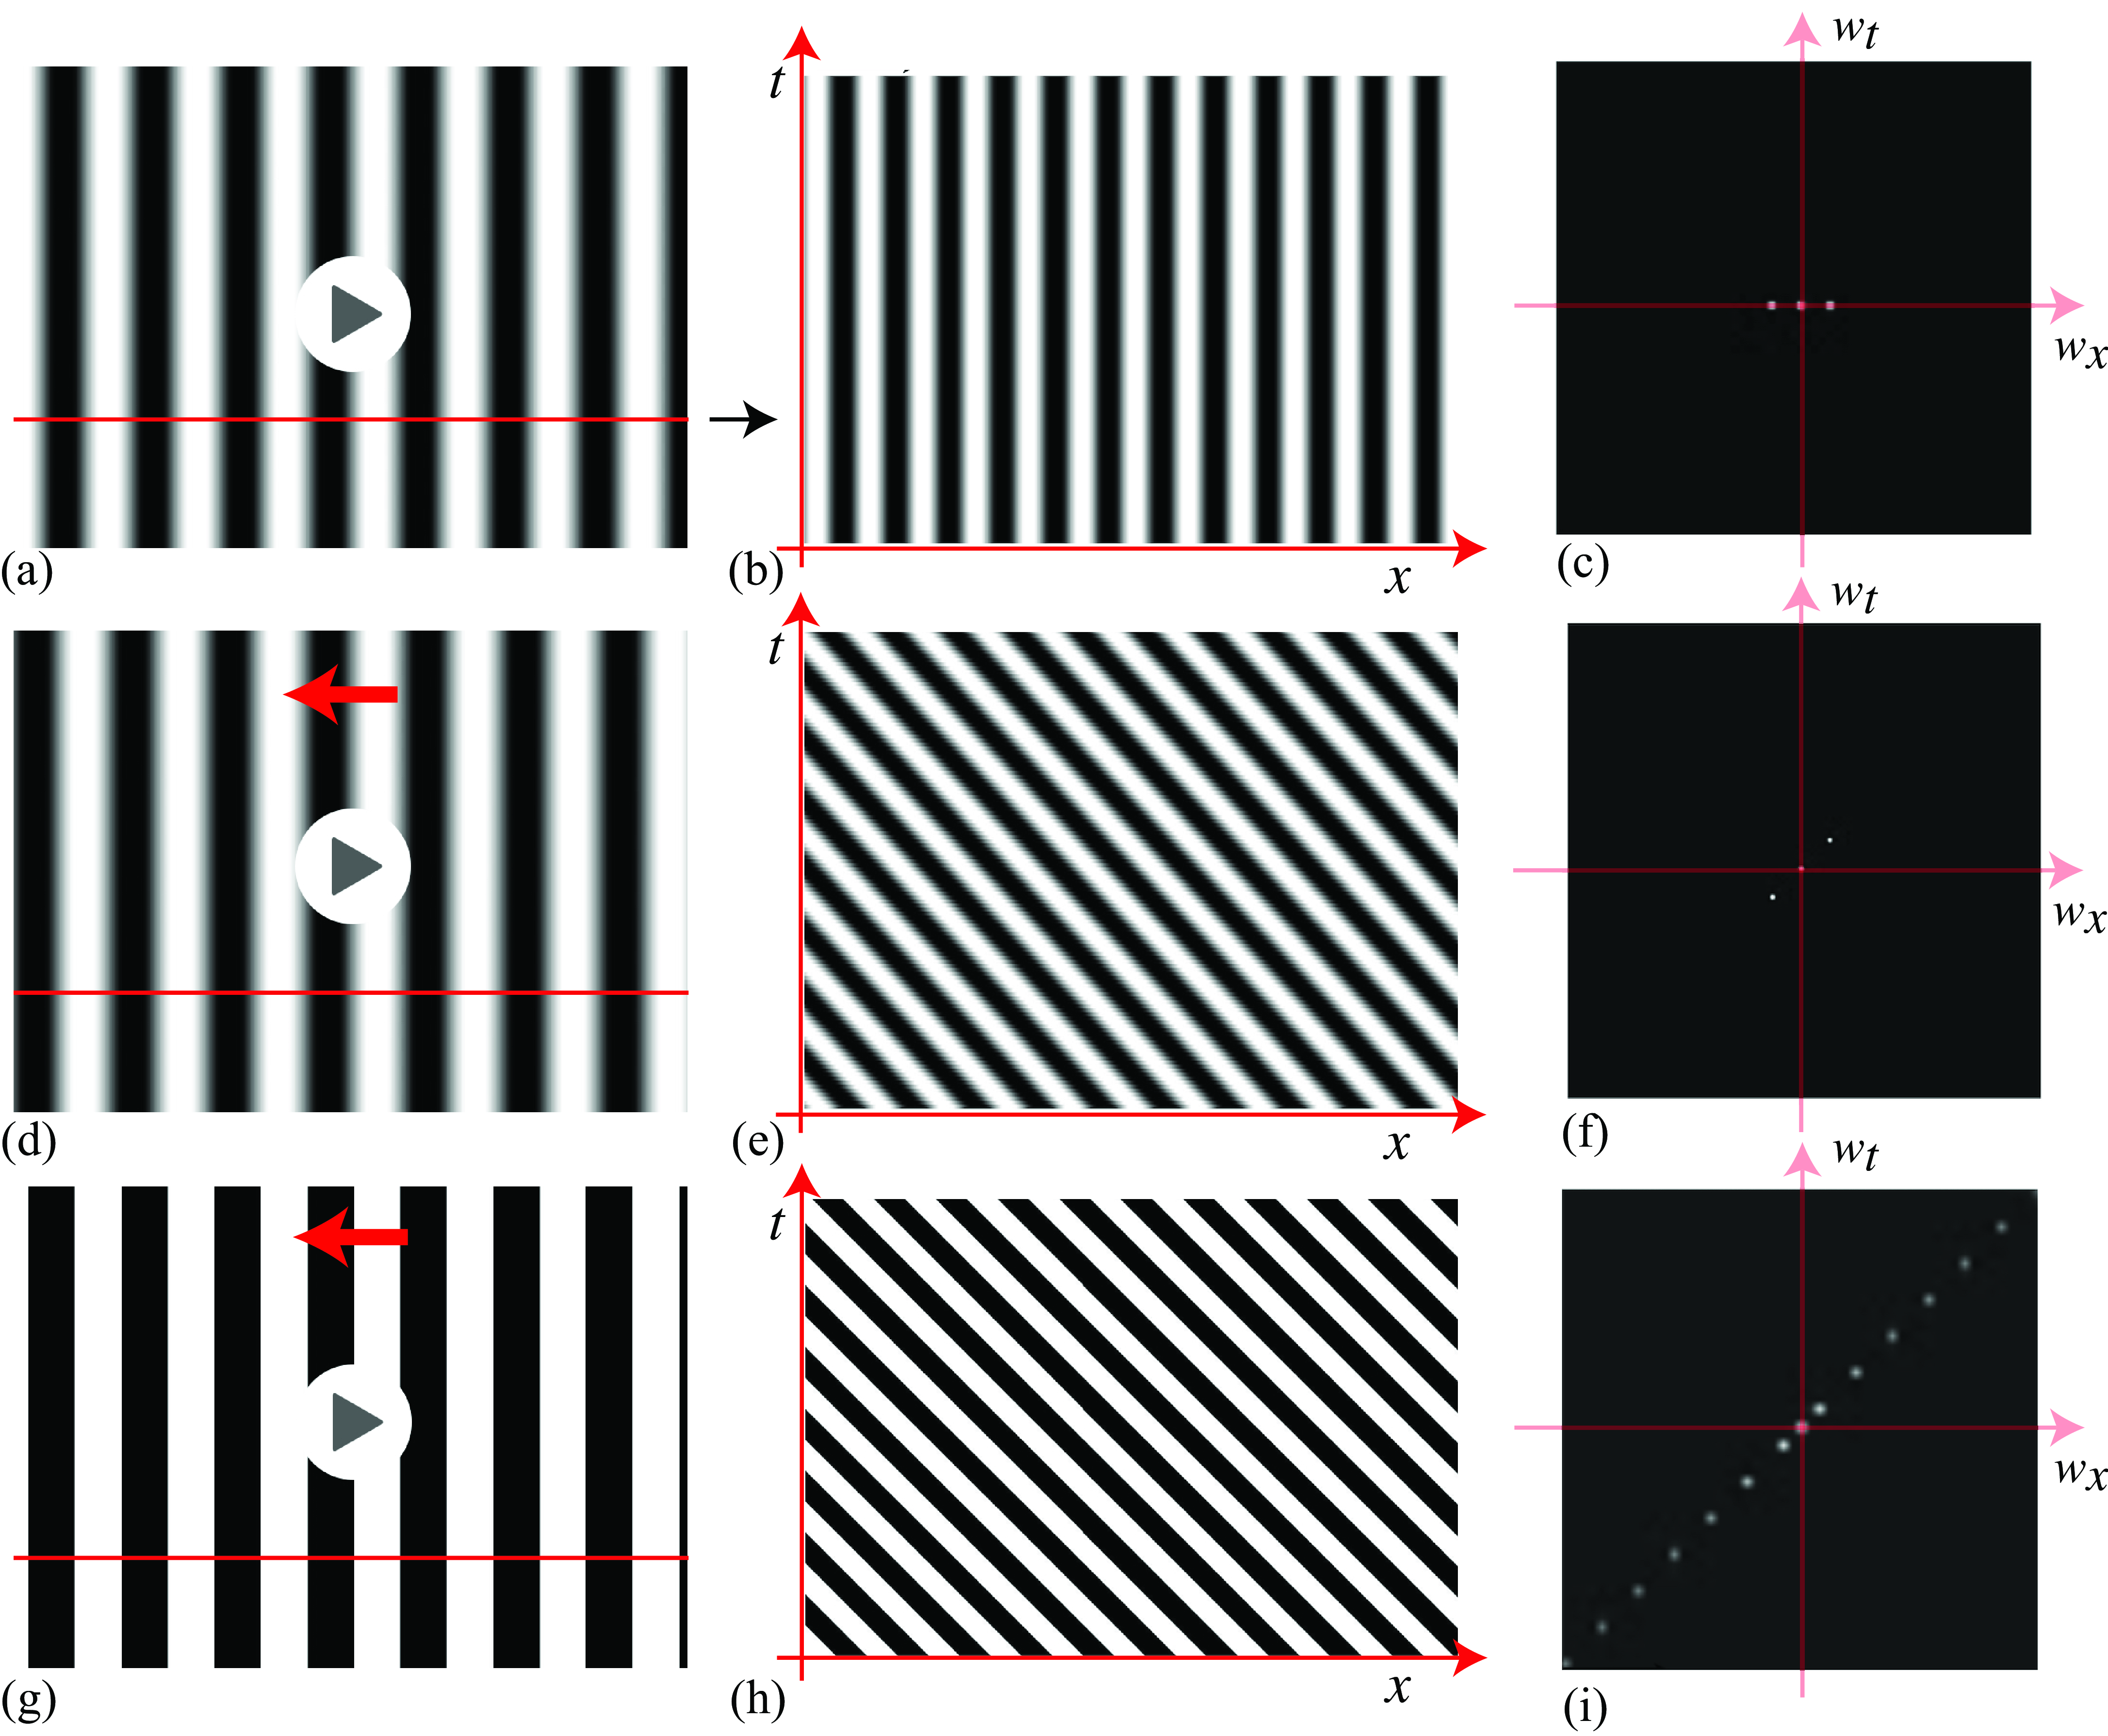
\includegraphics[width=1\linewidth]{figures/optical_flow/ted_demo_motion_1.eps}
    }
    %\centerline{
    %\hspace{-0.2in}
    %\sublabelnp{(a) 
    %\href{https://groups.csail.mit.edu/vision/cvbook/videos/stillsineLoop.mov}{stationary sine wave (click for video)}}
    %{
    %\href{https://groups.csail.mit.edu/vision/cvbook/videos/stillsineLoop.mov}{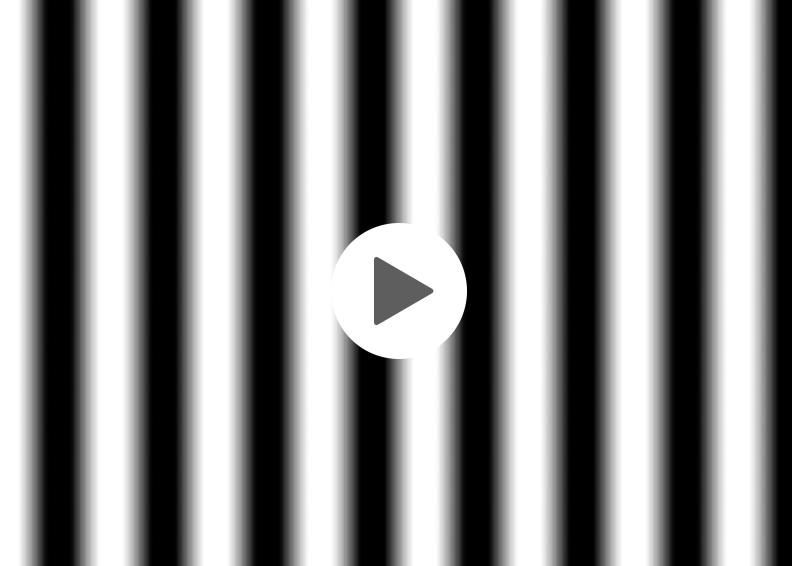
\includegraphics[width=0.2\linewidth]{figures/temporal_filters/movie1.jpg}}}
    %\sublabelnp{(b) space-time image}{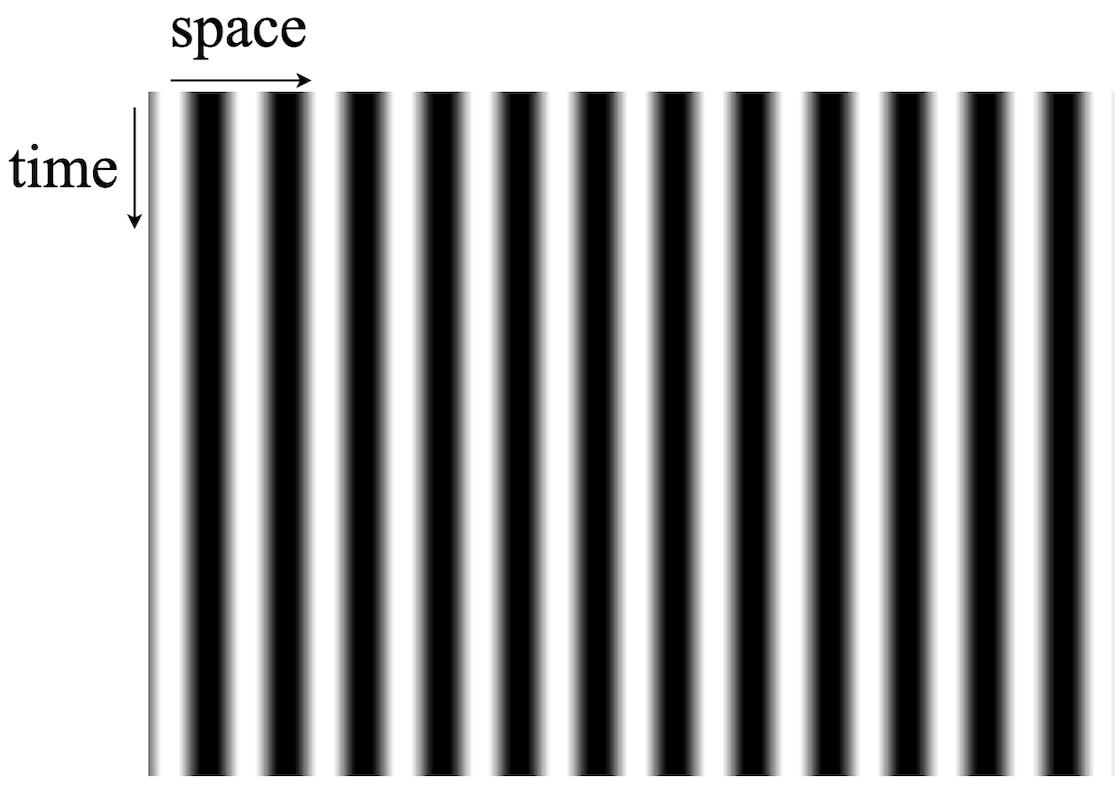
\includegraphics[width=0.3\linewidth]{figures/temporal_filters/st1a.jpg}}
    %\sublabelnp{(c) space-time Fourier transform}{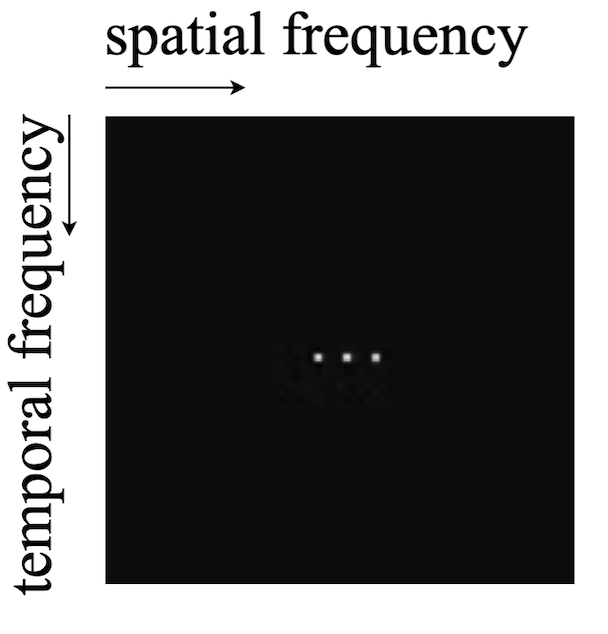
\includegraphics[width=0.3\linewidth]{figures/temporal_filters/stdft1.jpg}}}
    %\centerline{
    %\sublabelnp{(d) 
    %\href{https://groups.csail.mit.edu/vision/cvbook/videos/movingSineLoop.mov}{moving sine wave (click for video)}
    %}
    %{
    %\href{https://groups.csail.mit.edu/vision/cvbook/videos/movingSineLoop.mov}{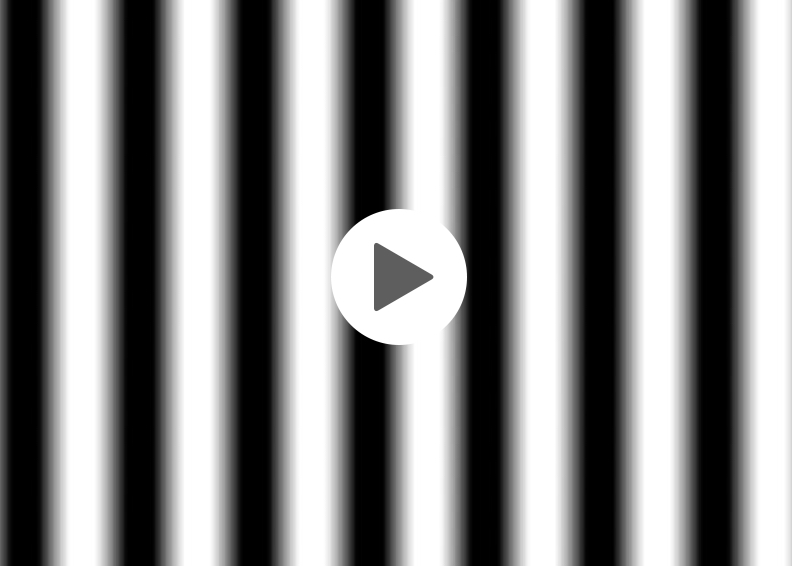
\includegraphics[width=0.2\linewidth]{figures/temporal_filters/movie2.jpg}}}
    %\hspace{0.1in}
    %\sublabelnp{(e) space-time image}{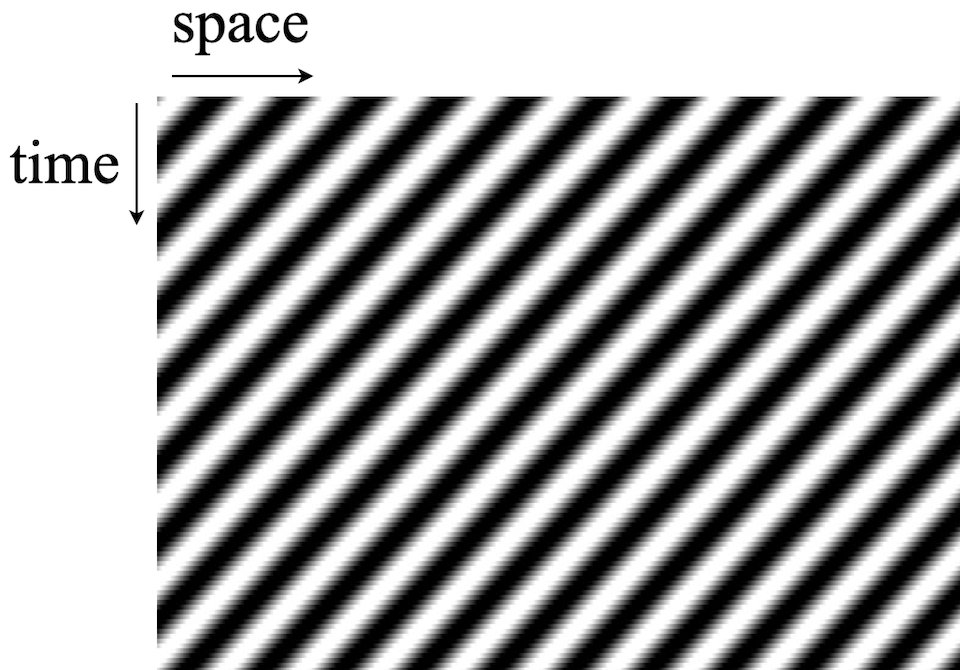
\includegraphics[width=0.3\linewidth]{figures/temporal_filters/st2.jpg}}
    %\hspace{0.5}
    %\sublabelnp{(f) space-time Fourier transform}{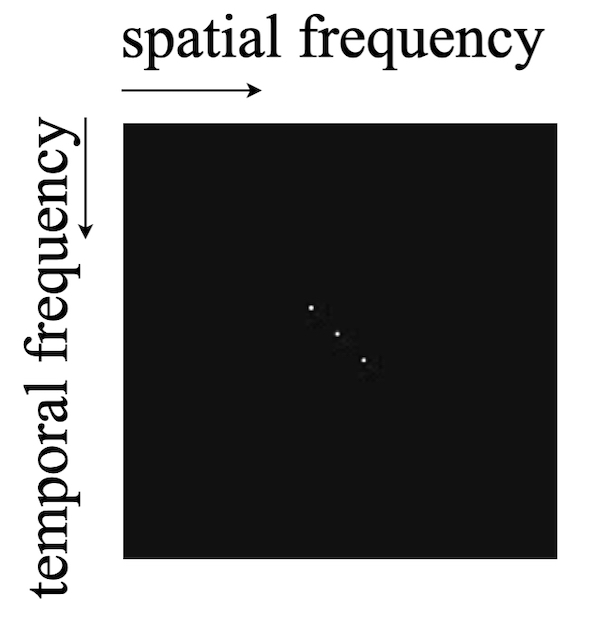
\includegraphics[width=0.3\linewidth]{figures/temporal_filters/stdft2.jpg}}
    %}
    %\centerline{
    %\sublabelnp{(g) 
    %\href{https://groups.csail.mit.edu/vision/cvbook/videos/movingSquareLoop.mov}{moving square wave (click for video)}
    %}
    %{
    %\href{https://groups.csail.mit.edu/vision/cvbook/videos/movingSquareLoop.mov}{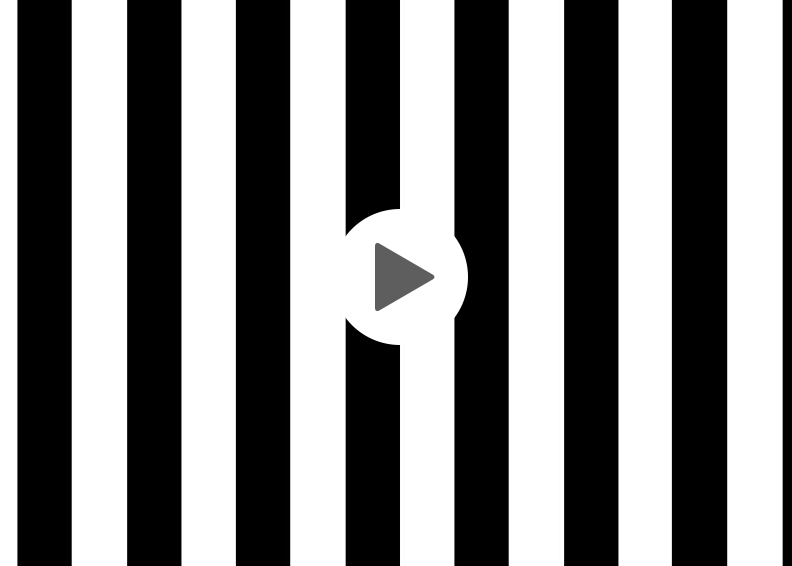
\includegraphics[width=0.2\linewidth]{figures/temporal_filters/movie3.jpg}}}
    %\hspace{-0.8}
    %\sublabelnp{(h) space-time Fourier transform}{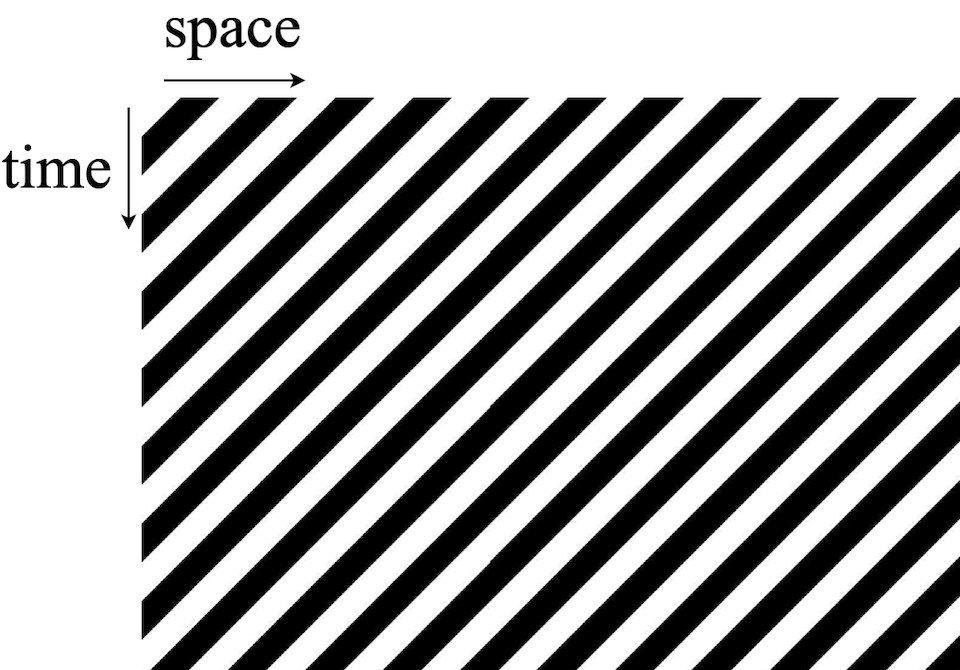
\includegraphics[width=0.3\linewidth]{figures/temporal_filters/st3.jpg}}
    %\hspace{-0.1in}
    %\sublabelnp{(i) space-time Fourier transform}{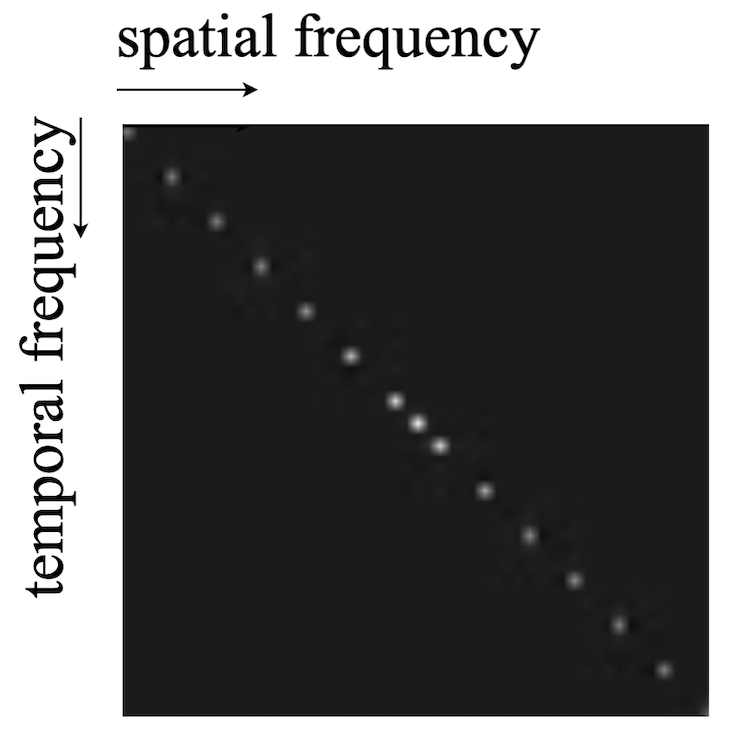
\includegraphics[width=0.3\linewidth]{figures/temporal_filters/stdft3.jpg}}
    %}
    \caption{Space-time signals, building toward the fluted square-wave motion illusion.    First row: stationary sine wave, (a) Movie of a motionless sine wave. (b) The space-time plot shows only vertical structure.
        (c) spatio-temporal Fourier transform has all energy on the zero temporal frequency axis, since nothing is moving.
        Second row:  (d) moving sine wave. (e) In the space-time plot, speed corresponds to local orientation. (f) The Fourier transform energy is sheared according to the sine wave's speed.
        Third row:  Moving square wave.  The additional harmonics required to form a square wave are visible in the spatio-temporal Fourier transform, (i).}
    \label{fig:motionIllusion1}
\end{figure}



\begin{figure}
    \centerline{
        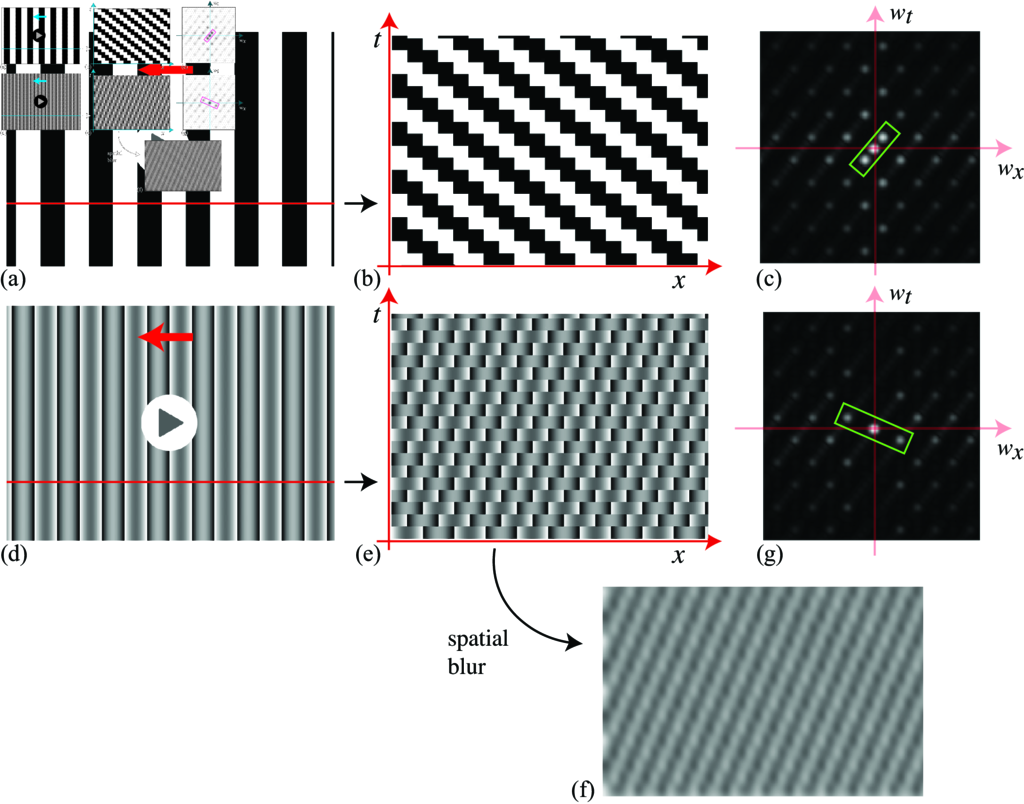
\includegraphics[width=1\linewidth]{figures/optical_flow/ted_demo_motion_2.eps}
    }
    \caption{Derivation of the fluted square-wave motion illusion, continued from Fig.~\ref{fig:motionIllusion1}.  First row:  This square wave moves in 1/4 wavelength jumps, instead of continuously.  This staggered motion generates the additional spatio-temporal frequencies shown in (a).  The lowest spatio-temporal frequency still indicates motion to the left.  Second row:  If we remove the lowest spatial frequency sine wave of the square wave, creating a "fluted square wave", then the lowest spatio-temporal frequency now moves in the other direction.  This is also visible from the space time plot in (e), and especially in the spatio-temporally low-pass filtered version, (f).}
    \label{fig:motionIllusion2}
\end{figure}



\begin{figure}
    \centerline{
        \sublabelnp{(a)
            \href{https://groups.csail.mit.edu/vision/cvbook/videos/blendedSlowLoop.mov}{motion illusion, slow (click for video)}
        }
        {
            \href{https://groups.csail.mit.edu/vision/cvbook/videos/blendedSlowLoop.mov}{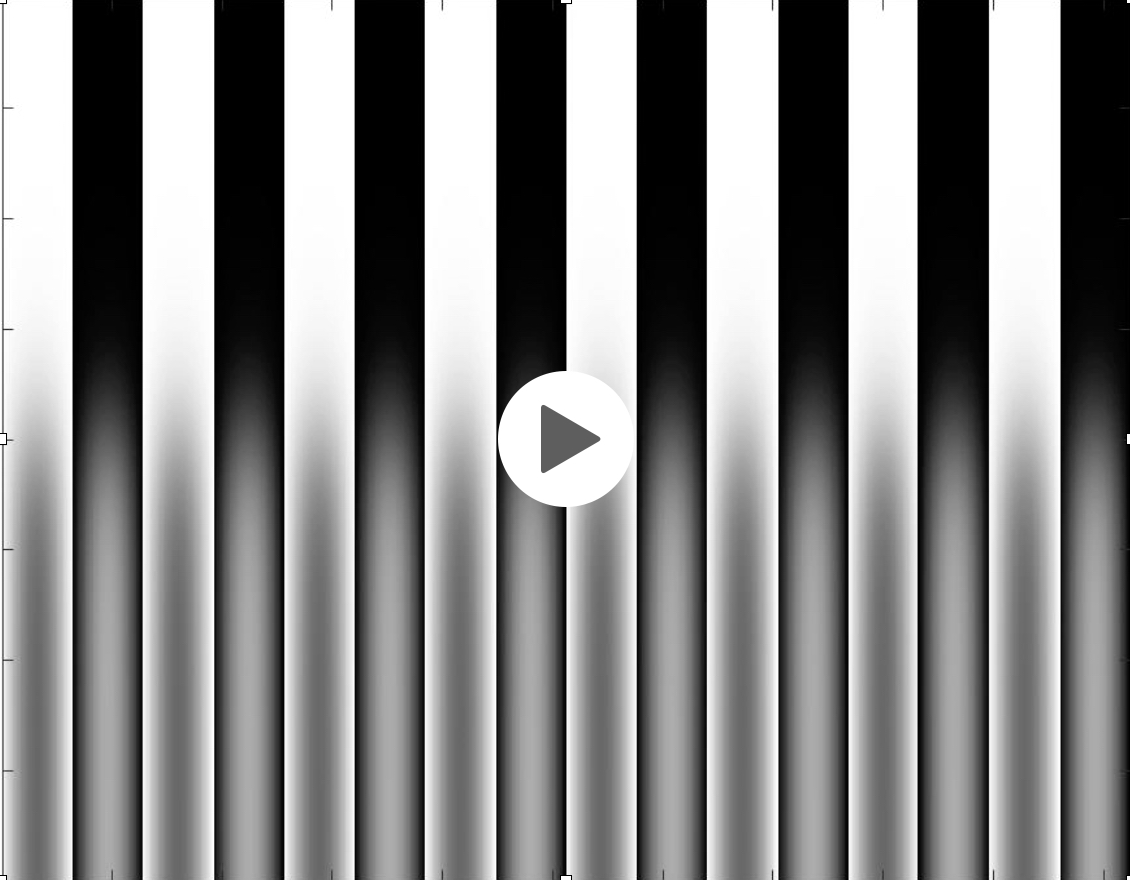
\includegraphics[width=0.5\linewidth]{figures/temporal_filters/blendFrame.jpg}}}
        \sublabelnp{(b)
            \href{https://groups.csail.mit.edu/vision/cvbook/videos/fastBlendLoop.mov}{motion illusion, fast (click for video)}
        }
        {
            \href{https://groups.csail.mit.edu/vision/cvbook/videos/fastBlendLoop.mov}{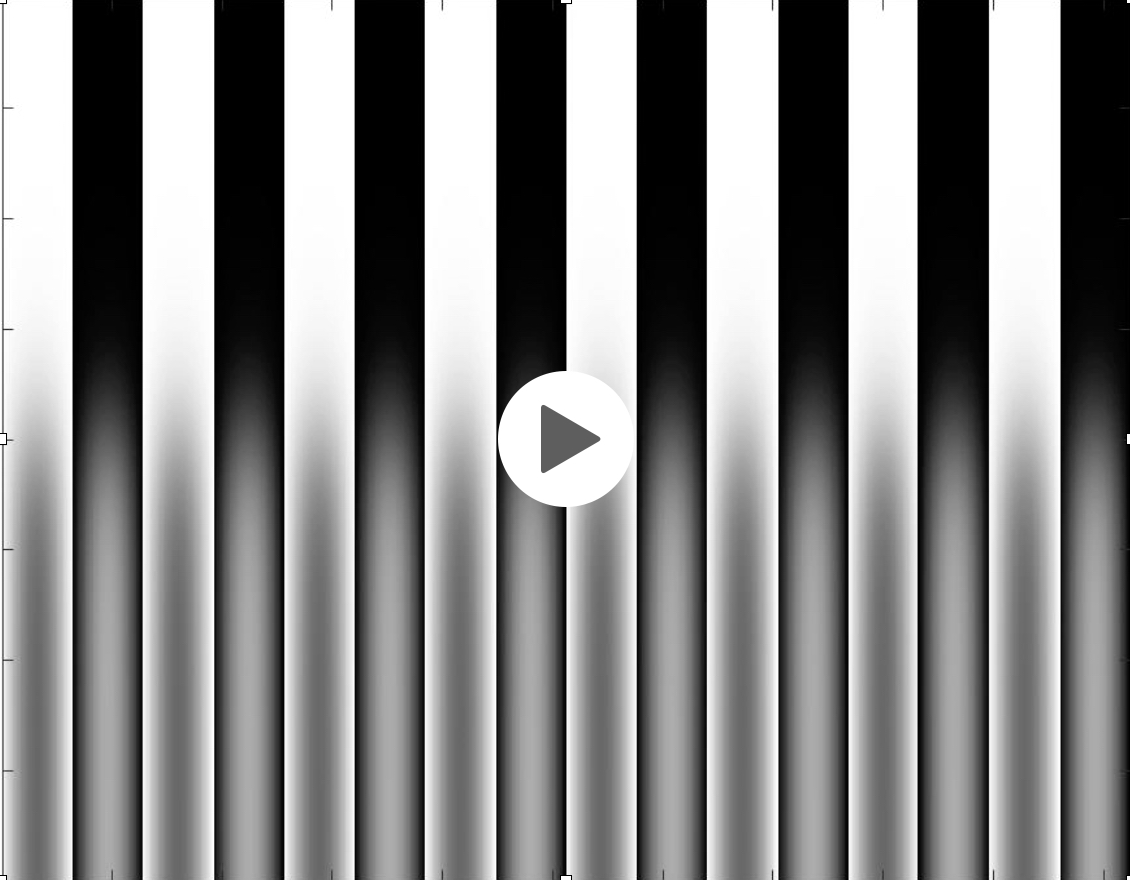
\includegraphics[width=0.5\linewidth]{figures/temporal_filters/blendFrame.jpg}}}
    }
    \caption{"Impossible combination" of ordinary and  fluted square-waves (view on looping display).  While one can verify, by tracing a finger or scanning your eyes, that the entire structure is moving rigidly to the left, the bottom half appears to be moving to the right.  At a fast speed, (b), the effect is accentuated.}
    \label{fig:blends}
\end{figure}



%Here's a mock-up of a real scene.  We have a stationary background,
%and two cars driving in opposite directions.  (Thanks to Anat Levin
%for creating this slide).
%
%
%\begin{figure}
%\centerline{
%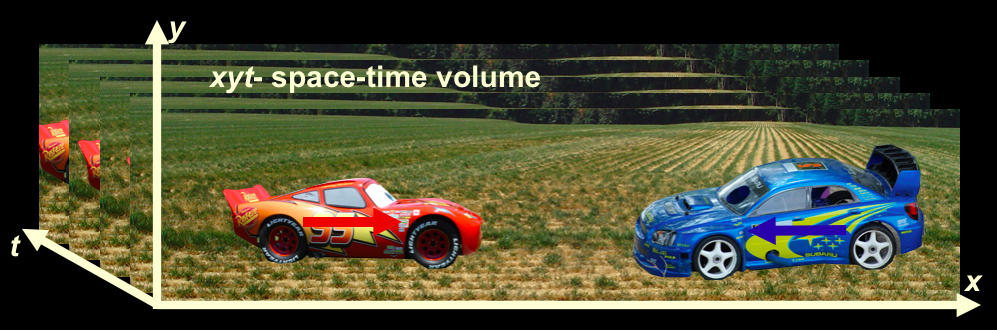
\includegraphics[width=0.6\linewidth]{figures/figs3/cars1.jpg}
%}
%\centerline{
%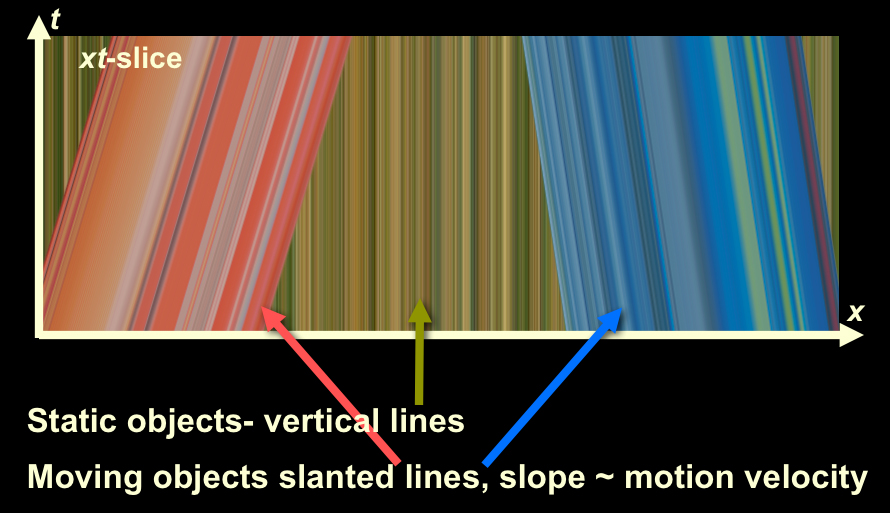
\includegraphics[width=0.6\linewidth]{figures/figs3/spacetime.jpg}
%}
%\caption{Top:  image sequence viewed as a space-time volume.  Bottom:
%The slope in a space-time plot indicates change in x per change in
%time, or the speed.}
%\label{fig:cars12}
%\end{figure}
%
%
%Let's consider the signal itself, Fig.~\ref{fig:cars12}.  Here
%is a 2-d slice of the volumetric video data of 2-d pixel intensities
%observed over time.  In our x-t slice we notice what we learn in
%elementary geometry classes:  the slope of the constant-intensity
%lines, change in time per change in x, indicate the speed of the
%observed pixels.  (This identification assumes constant pixel
%intensities over time).   So identifying the {\em speed} of objects in the
%image is equivalent to finding the {\em orientation} of structures in the
%spatio-temporal volume.  (In the full 3-d video volume, the 3-d
%orientation of constant pixel values indicates the {\em velocity} of
%motion).


%
%
%The fact that we find such space-time filters in neurophysiological
%studies of mammalian visual systems suggests that we may use such
%filter outputs in our own visual systems.  Let's look at a visual
%demonstration which addresses that question.  
%
%Consider a square wave.  From Fourier
%analysis, we know we can synthesize it from a sum of odd harmonics, as
%shown in the equation.  Each frequency comes in with an amplitude of
%$\frac{1}{\omega}$, where $\omega = 2 \pi f$ is its spatial frequency.  
%\begin{equation}
%x_{\mbox{square}}(t) = \frac{4}{\pi}(\sin(2 \pi f t) + \{frac{1}{3}
%\sin(6 \pi f t) + \frac{1}{5} \sin (10 \pi f t) + \hdots)
%\end{equation}
%
%
%Consider the following signal over time:  a square wave, translating
%$\frac{1}{4}$ cycle each frame of a movie.  The signal in space-time
%would look something like this.
%
%What are the different Fourier components of the square wave doing in
%this movie?  The fundamental sine wave has the same frequency as the
%square wave itself, so it, too, is jumping by $\frac{1}{4}$ of a cycle
%(or $90^\circ$) each frame.
%
%The next harmonic, $\frac{1}{3} \sin(3 \omega t)$ jumps by 
%$270^\circ$ each frame, or, equivalently, by $-90^\circ$.  It is
%aliased and, viewed in isolation, would appear to be moving in the
%other direction.
%
%What if we make a``fluted square wave'' signal, the same as
%the original square wave, but with the fundamental sinusoid, 
%$\sin(\omega t)$, subtracted out?  The signal would look like this, in
%space-time.
%
%\begin{figure}
%\centerline{
%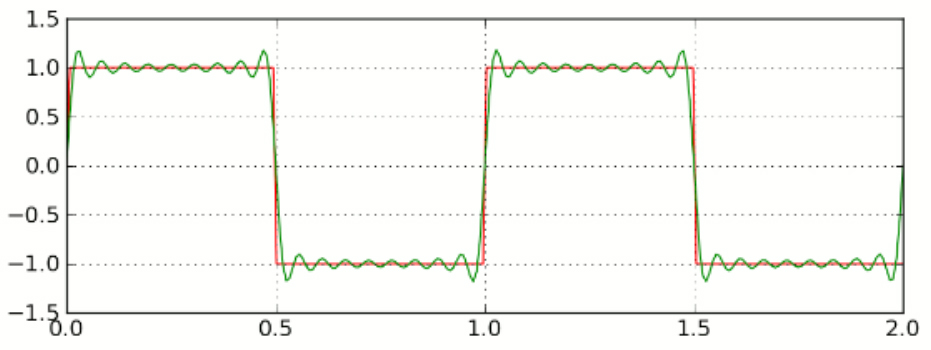
\includegraphics[width=0.8\linewidth]{figures/figs3/sinsquare.jpg}
%}
%\caption{approximation of square wave with sinusoids}
%\label{fig:squaresin}
%\end{figure}
%
%The question is, how would we perceive it moving?  The fluted square
%wave signal is really moving to the left, as the original sine wave
%was.  But the dominant sinusoidal component 
%(which is $\frac{1}{3} \sin(3 \omega t)$, after we remove the
%fundamental from the square wave), viewed in isolation, is moving to
%the right.
%
%\begin{figure}
%\centerline{
%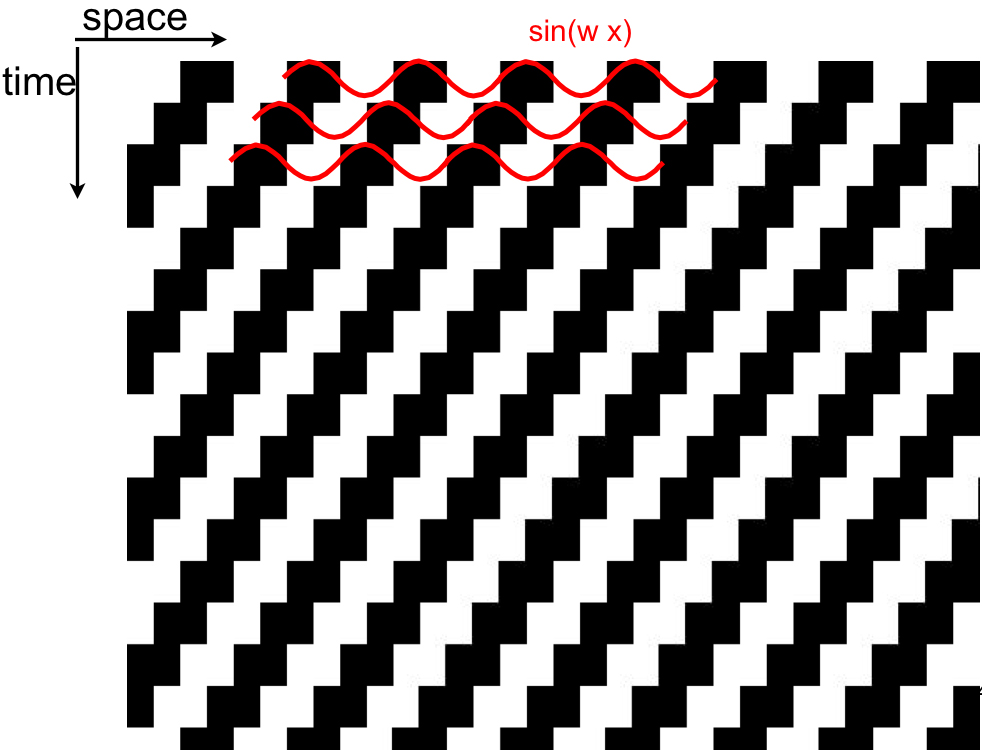
\includegraphics[width=0.6\linewidth]{figures/figs3/squaremotion.jpg}
%}
%\centerline{
%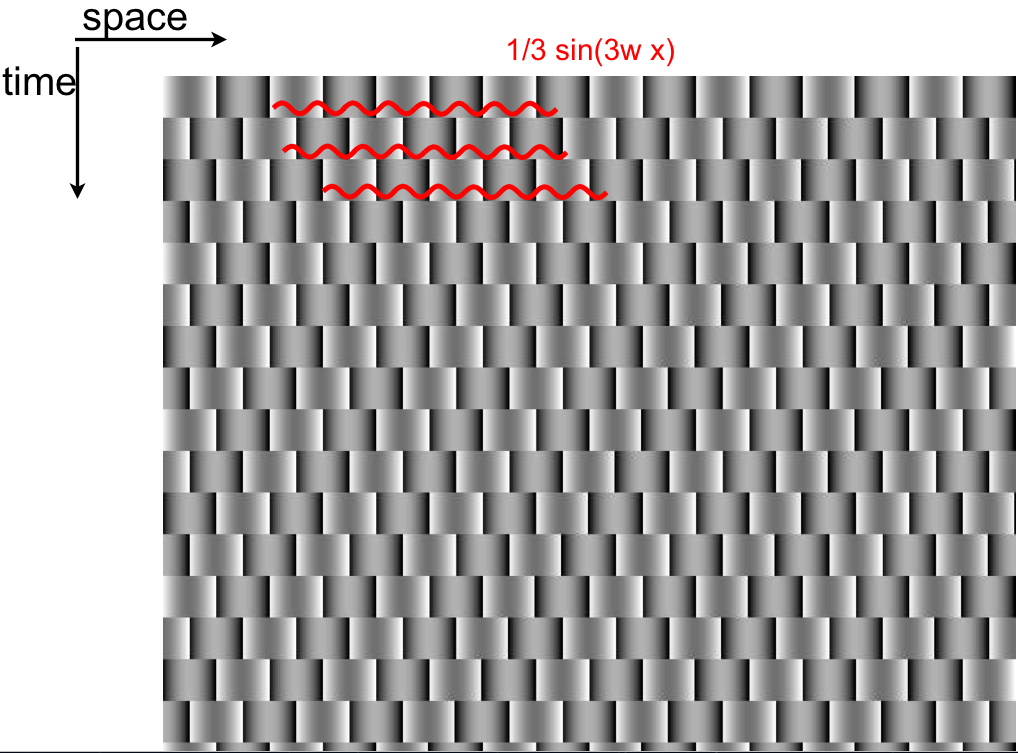
\includegraphics[width=0.6\linewidth]{figures/figs3/flutemotion.jpg}
%}
%\caption{motions}
%\label{fig:motions}
%\end{figure}
%
%
%So will we perceive the signal as an integral whole, and perceive it
%to be moving to the left?  Or will we perceive it as if through a
%federation of oriented filters, each one telling us, for the spatial
%frequency it is tuned to, what is the speed and direction with the
%most motion energy?  Will the visual system choose signal integrity,
%where it has to assimilate all the motion energy filter responses into
%a coherent story describing them all?  Or will it choose computational
%expedience and just listen to the spatio-temporal energy response that
%shouts the loudest?
%
%If we run the experiment, we find  the answer.  The visual
%system seems to take the easy (fast?) way out in this case, and signals
%to us which motion energy filter is responding the strongest:  the
%fluted square wave stimulus appears to be moving to the right.
%
%The quadrature pair motion energy filters, while very simple, are
%powerful enough to perform processing that mimics what a system as
%sophisticated as the human visual system does in some circumstances.
%
%
%\subsection{Motion magnification}
%
%This is an example of dealing with motion signals using filter-based approaches. There is no explicit measurement of motion per se: this method does not explicitly measures velocities.
%
%\begin{figure}
%\centerline{
%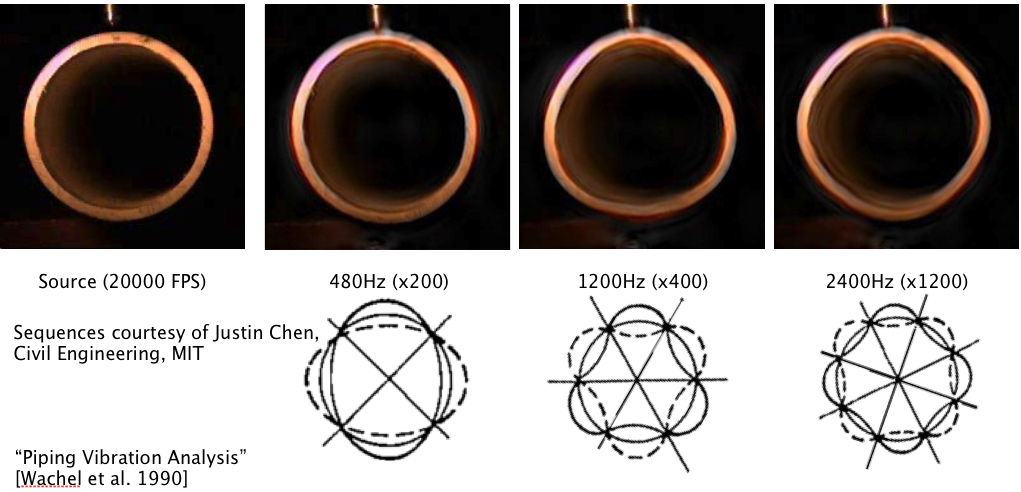
\includegraphics[width=0.8\linewidth]{figures/figs3/pipes.jpg}
%}
%\caption{Still frames of motion magnification output of high-speed
%  video of PVC pipe being struck by a hammer.
%}
%\label{fig:pipes}
%\end{figure}
%
%


%\subsection{The iris code}
%
%\begin{figure}
%\centerline{
%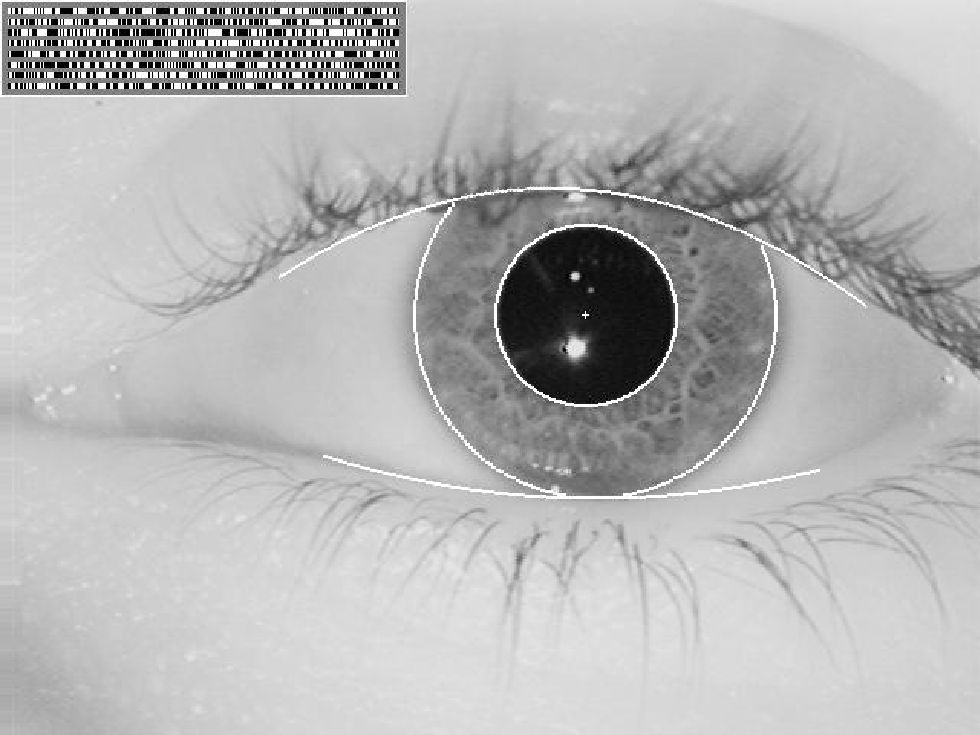
\includegraphics[width=0.4\linewidth]{figures/figs3/daugman1.pdf} 
%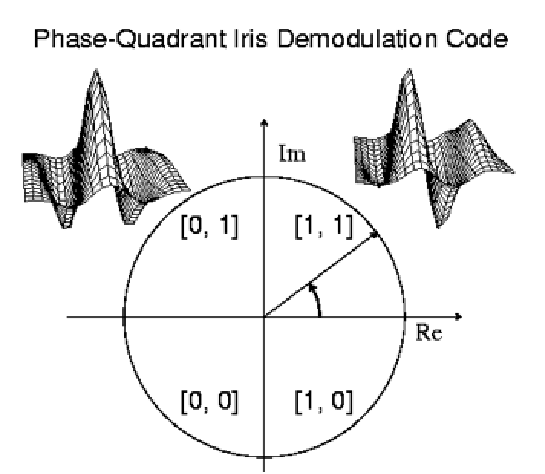
\includegraphics[width=0.4\linewidth]{figures/figs3/daugman2.pdf} 
%}
%\caption{Daugman} 
%\label{fig:daugman}
%\end{figure}
%
%Gabor filters (and indeed, quadrature pair filters in general)
%are useful for many things.   One use they've been put to is in
%quantifying the random textures of the human iris, developed by John
%Daugman, at Cambridge University.   The goal is to
%find a texture descriptor that is invariant to the various 
%conditions under which one might acquire an image of an eye.  The iris
%code measures the relative phase of a Gabor filter pair and quantifies
%that measurement into one of 4 bins (slide 119).  Of course, the
%filters must be aligned with the features of the eye, and
%concentrically oriented around the eye.  The result is a
%high-dimensional code for an individual's iris.  This code is able to
%ascertain identity with very high certainty (and immune to any issues
%with identical twins, because their irises develop under unique random
%processes).
%
%
%
